% Options for packages loaded elsewhere
\PassOptionsToPackage{unicode}{hyperref}
\PassOptionsToPackage{hyphens}{url}
%
\documentclass[
]{article}
\usepackage{amsmath,amssymb}
\usepackage{lmodern}
\usepackage{iftex}
\ifPDFTeX
  \usepackage[T1]{fontenc}
  \usepackage[utf8]{inputenc}
  \usepackage{textcomp} % provide euro and other symbols
\else % if luatex or xetex
  \usepackage{unicode-math}
  \defaultfontfeatures{Scale=MatchLowercase}
  \defaultfontfeatures[\rmfamily]{Ligatures=TeX,Scale=1}
\fi
% Use upquote if available, for straight quotes in verbatim environments
\IfFileExists{upquote.sty}{\usepackage{upquote}}{}
\IfFileExists{microtype.sty}{% use microtype if available
  \usepackage[]{microtype}
  \UseMicrotypeSet[protrusion]{basicmath} % disable protrusion for tt fonts
}{}
\makeatletter
\@ifundefined{KOMAClassName}{% if non-KOMA class
  \IfFileExists{parskip.sty}{%
    \usepackage{parskip}
  }{% else
    \setlength{\parindent}{0pt}
    \setlength{\parskip}{6pt plus 2pt minus 1pt}}
}{% if KOMA class
  \KOMAoptions{parskip=half}}
\makeatother
\usepackage{xcolor}
\usepackage[margin=1in]{geometry}
\usepackage{color}
\usepackage{fancyvrb}
\newcommand{\VerbBar}{|}
\newcommand{\VERB}{\Verb[commandchars=\\\{\}]}
\DefineVerbatimEnvironment{Highlighting}{Verbatim}{commandchars=\\\{\}}
% Add ',fontsize=\small' for more characters per line
\usepackage{framed}
\definecolor{shadecolor}{RGB}{248,248,248}
\newenvironment{Shaded}{\begin{snugshade}}{\end{snugshade}}
\newcommand{\AlertTok}[1]{\textcolor[rgb]{0.94,0.16,0.16}{#1}}
\newcommand{\AnnotationTok}[1]{\textcolor[rgb]{0.56,0.35,0.01}{\textbf{\textit{#1}}}}
\newcommand{\AttributeTok}[1]{\textcolor[rgb]{0.77,0.63,0.00}{#1}}
\newcommand{\BaseNTok}[1]{\textcolor[rgb]{0.00,0.00,0.81}{#1}}
\newcommand{\BuiltInTok}[1]{#1}
\newcommand{\CharTok}[1]{\textcolor[rgb]{0.31,0.60,0.02}{#1}}
\newcommand{\CommentTok}[1]{\textcolor[rgb]{0.56,0.35,0.01}{\textit{#1}}}
\newcommand{\CommentVarTok}[1]{\textcolor[rgb]{0.56,0.35,0.01}{\textbf{\textit{#1}}}}
\newcommand{\ConstantTok}[1]{\textcolor[rgb]{0.00,0.00,0.00}{#1}}
\newcommand{\ControlFlowTok}[1]{\textcolor[rgb]{0.13,0.29,0.53}{\textbf{#1}}}
\newcommand{\DataTypeTok}[1]{\textcolor[rgb]{0.13,0.29,0.53}{#1}}
\newcommand{\DecValTok}[1]{\textcolor[rgb]{0.00,0.00,0.81}{#1}}
\newcommand{\DocumentationTok}[1]{\textcolor[rgb]{0.56,0.35,0.01}{\textbf{\textit{#1}}}}
\newcommand{\ErrorTok}[1]{\textcolor[rgb]{0.64,0.00,0.00}{\textbf{#1}}}
\newcommand{\ExtensionTok}[1]{#1}
\newcommand{\FloatTok}[1]{\textcolor[rgb]{0.00,0.00,0.81}{#1}}
\newcommand{\FunctionTok}[1]{\textcolor[rgb]{0.00,0.00,0.00}{#1}}
\newcommand{\ImportTok}[1]{#1}
\newcommand{\InformationTok}[1]{\textcolor[rgb]{0.56,0.35,0.01}{\textbf{\textit{#1}}}}
\newcommand{\KeywordTok}[1]{\textcolor[rgb]{0.13,0.29,0.53}{\textbf{#1}}}
\newcommand{\NormalTok}[1]{#1}
\newcommand{\OperatorTok}[1]{\textcolor[rgb]{0.81,0.36,0.00}{\textbf{#1}}}
\newcommand{\OtherTok}[1]{\textcolor[rgb]{0.56,0.35,0.01}{#1}}
\newcommand{\PreprocessorTok}[1]{\textcolor[rgb]{0.56,0.35,0.01}{\textit{#1}}}
\newcommand{\RegionMarkerTok}[1]{#1}
\newcommand{\SpecialCharTok}[1]{\textcolor[rgb]{0.00,0.00,0.00}{#1}}
\newcommand{\SpecialStringTok}[1]{\textcolor[rgb]{0.31,0.60,0.02}{#1}}
\newcommand{\StringTok}[1]{\textcolor[rgb]{0.31,0.60,0.02}{#1}}
\newcommand{\VariableTok}[1]{\textcolor[rgb]{0.00,0.00,0.00}{#1}}
\newcommand{\VerbatimStringTok}[1]{\textcolor[rgb]{0.31,0.60,0.02}{#1}}
\newcommand{\WarningTok}[1]{\textcolor[rgb]{0.56,0.35,0.01}{\textbf{\textit{#1}}}}
\usepackage{graphicx}
\makeatletter
\def\maxwidth{\ifdim\Gin@nat@width>\linewidth\linewidth\else\Gin@nat@width\fi}
\def\maxheight{\ifdim\Gin@nat@height>\textheight\textheight\else\Gin@nat@height\fi}
\makeatother
% Scale images if necessary, so that they will not overflow the page
% margins by default, and it is still possible to overwrite the defaults
% using explicit options in \includegraphics[width, height, ...]{}
\setkeys{Gin}{width=\maxwidth,height=\maxheight,keepaspectratio}
% Set default figure placement to htbp
\makeatletter
\def\fps@figure{htbp}
\makeatother
\setlength{\emergencystretch}{3em} % prevent overfull lines
\providecommand{\tightlist}{%
  \setlength{\itemsep}{0pt}\setlength{\parskip}{0pt}}
\setcounter{secnumdepth}{-\maxdimen} % remove section numbering
\ifLuaTeX
  \usepackage{selnolig}  % disable illegal ligatures
\fi
\IfFileExists{bookmark.sty}{\usepackage{bookmark}}{\usepackage{hyperref}}
\IfFileExists{xurl.sty}{\usepackage{xurl}}{} % add URL line breaks if available
\urlstyle{same} % disable monospaced font for URLs
\hypersetup{
  hidelinks,
  pdfcreator={LaTeX via pandoc}}

\author{}
\date{\vspace{-2.5em}}

\begin{document}

\hypertarget{convolutional-neural-networks-with-webscrapping-in-python}{%
\section{Convolutional Neural Networks with webscrapping in
Python}\label{convolutional-neural-networks-with-webscrapping-in-python}}

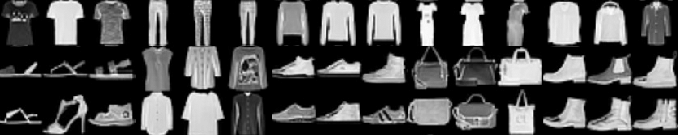
\includegraphics{02_fashionmnist.png}

\hypertarget{set-up---load-libraries}{%
\subsection{Set up - load libraries}\label{set-up---load-libraries}}

\begin{Shaded}
\begin{Highlighting}[]
\CommentTok{\# R libraries}
\CommentTok{\# Deep learning}
\NormalTok{tensorflow}\SpecialCharTok{::}\FunctionTok{install\_tensorflow}\NormalTok{()}
\end{Highlighting}
\end{Shaded}

\begin{verbatim}
## Using virtual environment "~/.virtualenvs/r-reticulate" ...
## 
## Installation complete.
\end{verbatim}

\begin{Shaded}
\begin{Highlighting}[]
\FunctionTok{library}\NormalTok{(keras)}
\FunctionTok{library}\NormalTok{(tensorflow)}

\CommentTok{\# Data wrangling}
\FunctionTok{library}\NormalTok{(tidyverse)}

\CommentTok{\# Image manipulation}
\FunctionTok{library}\NormalTok{(imager)}

\CommentTok{\# Model Evaluation}
\FunctionTok{library}\NormalTok{(caret)}
\end{Highlighting}
\end{Shaded}

\begin{Shaded}
\begin{Highlighting}[]
\CommentTok{\# Python libraries}
\ImportTok{from}\NormalTok{ bs4 }\ImportTok{import}\NormalTok{ BeautifulSoup}
\ImportTok{import}\NormalTok{ requests}
\ImportTok{import}\NormalTok{ time}
\ImportTok{import}\NormalTok{ random}
\ImportTok{import}\NormalTok{ pickle}
\ImportTok{import}\NormalTok{ shutil}
\ImportTok{import}\NormalTok{ os}
\end{Highlighting}
\end{Shaded}

\hypertarget{data}{%
\subsection{Data}\label{data}}

Data set of \ldots{} pictures downloaded from www.grzyby.pl.

\hfill\break

\hypertarget{web-scrap-with-python}{%
\subsection{Web scrap with Python}\label{web-scrap-with-python}}

Initial settings - edibility classes.

\begin{Shaded}
\begin{Highlighting}[]
\CommentTok{\# Edibility lists}
\NormalTok{elements }\OperatorTok{=}\NormalTok{ [}\StringTok{\textquotesingle{}🟢!\textquotesingle{}}\NormalTok{,}\StringTok{\textquotesingle{}🟢\textquotesingle{}}\NormalTok{,}\StringTok{\textquotesingle{}🟡🟢\textquotesingle{}}\NormalTok{,}\StringTok{\textquotesingle{}🟡\textquotesingle{}}\NormalTok{,}\StringTok{\textquotesingle{}🔴\textquotesingle{}}\NormalTok{,}\StringTok{\textquotesingle{}🔴☠\textquotesingle{}}\NormalTok{]}

\NormalTok{edible }\OperatorTok{=}\NormalTok{ [}\StringTok{\textquotesingle{}🟢!\textquotesingle{}}\NormalTok{,}\StringTok{\textquotesingle{}🟢\textquotesingle{}}\NormalTok{]}
\NormalTok{non\_edible }\OperatorTok{=}\NormalTok{ [}\StringTok{\textquotesingle{}🟡🟢\textquotesingle{}}\NormalTok{,}\StringTok{\textquotesingle{}🟡\textquotesingle{}}\NormalTok{]}
\NormalTok{deadly }\OperatorTok{=}\NormalTok{ [}\StringTok{\textquotesingle{}🔴\textquotesingle{}}\NormalTok{,}\StringTok{\textquotesingle{}🔴☠\textquotesingle{}}\NormalTok{]}

\CommentTok{\# Edibility dict}
\NormalTok{edibility }\OperatorTok{=}\NormalTok{ \{}\StringTok{\textquotesingle{}edible\textquotesingle{}}\NormalTok{:[}\StringTok{\textquotesingle{}🟢!\textquotesingle{}}\NormalTok{,}\StringTok{\textquotesingle{}🟢\textquotesingle{}}\NormalTok{],}\StringTok{\textquotesingle{}non\_edible\textquotesingle{}}\NormalTok{:[}\StringTok{\textquotesingle{}🟡🟢\textquotesingle{}}\NormalTok{,}\StringTok{\textquotesingle{}🟡\textquotesingle{}}\NormalTok{],}\StringTok{\textquotesingle{}deadly\textquotesingle{}}\NormalTok{:[}\StringTok{\textquotesingle{}🔴\textquotesingle{}}\NormalTok{,}\StringTok{\textquotesingle{}🔴☠\textquotesingle{}}\NormalTok{]\}}
\end{Highlighting}
\end{Shaded}

Create 2 lists:

\begin{itemize}
\item
  mushroom names (in format `Amanita\_echinocephala')
\item
  mushroom webpages (in format
  `\url{https://grzyby.pl/pelna/gatunki/Amanita_echinocephala}')
\end{itemize}

\begin{Shaded}
\begin{Highlighting}[]
\CommentTok{\# Credentials to use full page functionality}
\NormalTok{credentials }\OperatorTok{=} \BuiltInTok{dict}\NormalTok{(l.rstrip().split(}\StringTok{\textquotesingle{}=\textquotesingle{}}\NormalTok{) }\ControlFlowTok{for}\NormalTok{ l }\KeywordTok{in} \BuiltInTok{open}\NormalTok{(}\StringTok{\textquotesingle{}config.properties\textquotesingle{}}\NormalTok{) }\ControlFlowTok{if} \KeywordTok{not}\NormalTok{ l.startswith(}\StringTok{"\#"}\NormalTok{))}
\NormalTok{URL\_init }\OperatorTok{=} \StringTok{"https://www.grzyby.pl/logowanie"}

\CommentTok{\# Log in using credential}
\NormalTok{form\_data }\OperatorTok{=}\NormalTok{ credentials}
\NormalTok{s }\OperatorTok{=}\NormalTok{ requests.Session()}
\NormalTok{server }\OperatorTok{=}\NormalTok{ s.post(URL\_init, data }\OperatorTok{=}\NormalTok{ form\_data)}

\CommentTok{\# Get full list of species}
\NormalTok{URL }\OperatorTok{=} \StringTok{\textquotesingle{}https://www.grzyby.pl/pelna/gatunki/\textquotesingle{}}
\NormalTok{page }\OperatorTok{=}\NormalTok{ s.get(URL)}
\NormalTok{soup }\OperatorTok{=}\NormalTok{ BeautifulSoup(page.content, }\StringTok{"html.parser"}\NormalTok{)}

\NormalTok{mushroom\_names }\OperatorTok{=}\NormalTok{ []}
\NormalTok{mushroom\_webs }\OperatorTok{=}\NormalTok{ []}
\ControlFlowTok{for}\NormalTok{ item }\KeywordTok{in}\NormalTok{ soup.find\_all(}\StringTok{\textquotesingle{}td\textquotesingle{}}\NormalTok{):}
    \ControlFlowTok{if}\NormalTok{ item.find(}\StringTok{\textquotesingle{}a\textquotesingle{}}\NormalTok{, href }\OperatorTok{=} \VariableTok{True}\NormalTok{) }\KeywordTok{and} \StringTok{\textquotesingle{}\_\textquotesingle{}} \KeywordTok{in} \BuiltInTok{str}\NormalTok{(item) }\KeywordTok{and} \StringTok{\textquotesingle{}{-}\textquotesingle{}} \KeywordTok{not} \KeywordTok{in} \BuiltInTok{str}\NormalTok{(item):}
\NormalTok{        name }\OperatorTok{=}\NormalTok{ item.find(}\StringTok{\textquotesingle{}a\textquotesingle{}}\NormalTok{).text}
\NormalTok{        name\_clean }\OperatorTok{=}\NormalTok{ item.find(}\StringTok{\textquotesingle{}a\textquotesingle{}}\NormalTok{).text.replace(}\StringTok{\textquotesingle{}.htm\textquotesingle{}}\NormalTok{, }\StringTok{\textquotesingle{}\textquotesingle{}}\NormalTok{)}
        \ControlFlowTok{if} \BuiltInTok{len}\NormalTok{(name\_clean.split(}\StringTok{\textquotesingle{}\_\textquotesingle{}}\NormalTok{)) }\OperatorTok{==} \DecValTok{2}\NormalTok{:}
\NormalTok{            mushroom\_webs.append(}\StringTok{\textquotesingle{}https://grzyby.pl/pelna/gatunki/\textquotesingle{}}\OperatorTok{+}\NormalTok{name)}
\NormalTok{            mushroom\_names.append(name\_clean)}

\BuiltInTok{print}\NormalTok{(}\SpecialStringTok{f\textquotesingle{}Lenght of mushroom\_names: }\SpecialCharTok{\{}\BuiltInTok{len}\NormalTok{(mushroom\_names)}\SpecialCharTok{\}}\SpecialStringTok{.}\CharTok{\textbackslash{}n}\SpecialStringTok{Lenght of mushroom\_webs: }\SpecialCharTok{\{}\BuiltInTok{len}\NormalTok{(mushroom\_webs)}\SpecialCharTok{\}}\SpecialStringTok{.\textquotesingle{}}\NormalTok{)}
\end{Highlighting}
\end{Shaded}

\begin{verbatim}
## Lenght of mushroom_names: 4909.
## Lenght of mushroom_webs: 4909.
\end{verbatim}

\hypertarget{create-functions-to-download-pictures}{%
\subsection{Create functions to download
pictures}\label{create-functions-to-download-pictures}}

\hypertarget{function-to-create-dictionary-from-given-lists}{%
\subsubsection{Function to create dictionary from given
lists}\label{function-to-create-dictionary-from-given-lists}}

\begin{Shaded}
\begin{Highlighting}[]
\CommentTok{\# name {-} name of dictionary}
\CommentTok{\# l\_names {-} list with mushroom names}
\CommentTok{\# l\_webs {-} list with mushroom websites}

\KeywordTok{def}\NormalTok{ mushroom\_dict\_init(l\_names:}\BuiltInTok{list}\NormalTok{, l\_webs:}\BuiltInTok{list}\NormalTok{, name:}\BuiltInTok{str}\OperatorTok{=}\StringTok{\textquotesingle{}\textquotesingle{}}\NormalTok{):}
    \ControlFlowTok{try}\NormalTok{:}
\NormalTok{        mushroom\_dict }\OperatorTok{=}\NormalTok{ \{l\_names[i]: \{}\StringTok{\textquotesingle{}edible\textquotesingle{}}\NormalTok{: }\VariableTok{None}\NormalTok{, }\StringTok{\textquotesingle{}web\textquotesingle{}}\NormalTok{: l\_webs[i], }\StringTok{\textquotesingle{}img\textquotesingle{}}\NormalTok{ : []\} }\ControlFlowTok{for}\NormalTok{ i }\KeywordTok{in} \BuiltInTok{range}\NormalTok{(}\BuiltInTok{len}\NormalTok{(l\_names))\}}

        \ControlFlowTok{if}\NormalTok{ name }\OperatorTok{!=} \StringTok{\textquotesingle{}\textquotesingle{}}\NormalTok{:}
\NormalTok{            mushroom\_dict[}\StringTok{\textquotesingle{}dict\_name\textquotesingle{}}\NormalTok{] }\OperatorTok{=}\NormalTok{ (}\SpecialStringTok{f\textquotesingle{}mushroom\_dict\_}\SpecialCharTok{\{}\NormalTok{name}\SpecialCharTok{\}}\SpecialStringTok{\textquotesingle{}}\NormalTok{)}
        \ControlFlowTok{else}\NormalTok{:}
\NormalTok{            mushroom\_dict[}\StringTok{\textquotesingle{}dict\_name\textquotesingle{}}\NormalTok{] }\OperatorTok{=}\NormalTok{ (}\SpecialStringTok{f\textquotesingle{}mushroom\_dict\textquotesingle{}}\NormalTok{)}

        \BuiltInTok{print}\NormalTok{(}\SpecialStringTok{f\textquotesingle{}Created }\SpecialCharTok{\{}\NormalTok{mushroom\_dict[}\StringTok{"dict\_name"}\NormalTok{]}\SpecialCharTok{\}}\SpecialStringTok{ with }\SpecialCharTok{\{}\BuiltInTok{len}\NormalTok{(mushroom\_dict)}\SpecialCharTok{\}}\SpecialStringTok{ elements.\textquotesingle{}}\NormalTok{)}
        \ControlFlowTok{return}\NormalTok{ mushroom\_dict}

    \ControlFlowTok{except} \PreprocessorTok{Exception} \ImportTok{as}\NormalTok{ e:}
        \BuiltInTok{print}\NormalTok{(}\SpecialStringTok{f\textquotesingle{}ERROR {-} not possible to create dictionary: }\SpecialCharTok{\{}\NormalTok{e}\SpecialCharTok{\}}\SpecialStringTok{.\textquotesingle{}}\NormalTok{)}
\end{Highlighting}
\end{Shaded}

\hypertarget{function-to-create-short-dictionary-for-tests}{%
\subsubsection{Function to create short dictionary for
tests}\label{function-to-create-short-dictionary-for-tests}}

\begin{Shaded}
\begin{Highlighting}[]
\CommentTok{\# name {-} name of dictionary}
\CommentTok{\# l\_names {-} list with mushroom names}
\CommentTok{\# l\_webs {-} list with mushroom websites}
\CommentTok{\# l\_mushs {-} list with expected families to be included in final dictionary}

\KeywordTok{def}\NormalTok{ mushroom\_dict\_short\_init(l\_names:}\BuiltInTok{list}\NormalTok{, l\_webs:}\BuiltInTok{list}\NormalTok{, l\_mushs:}\BuiltInTok{list}\NormalTok{, name:}\BuiltInTok{str}\OperatorTok{=}\StringTok{\textquotesingle{}\textquotesingle{}}\NormalTok{):}
\NormalTok{    l\_names\_short }\OperatorTok{=}\NormalTok{ []}
\NormalTok{    l\_webs\_short }\OperatorTok{=}\NormalTok{ []}

    \ControlFlowTok{try}\NormalTok{:}
        \ControlFlowTok{for}\NormalTok{ mushroom\_name }\KeywordTok{in}\NormalTok{ l\_names:}
            \ControlFlowTok{for}\NormalTok{ el }\KeywordTok{in}\NormalTok{ l\_mushs:}
                \ControlFlowTok{if}\NormalTok{ el }\KeywordTok{in}\NormalTok{ mushroom\_name:}
\NormalTok{                    l\_names\_short.append(mushroom\_name)}

        \ControlFlowTok{for}\NormalTok{ mushroom\_web }\KeywordTok{in}\NormalTok{ l\_webs:}
            \ControlFlowTok{for}\NormalTok{ el }\KeywordTok{in}\NormalTok{ l\_mushs:}
                \ControlFlowTok{if}\NormalTok{ el }\KeywordTok{in}\NormalTok{ mushroom\_web:}
\NormalTok{                    l\_webs\_short.append(mushroom\_web)}

\NormalTok{        mushroom\_dict\_short }\OperatorTok{=}\NormalTok{ \{l\_names\_short[i]: \{}\StringTok{\textquotesingle{}edible\textquotesingle{}}\NormalTok{: }\VariableTok{None}\NormalTok{, }\StringTok{\textquotesingle{}web\textquotesingle{}}\NormalTok{: l\_webs\_short[i], }\StringTok{\textquotesingle{}img\textquotesingle{}}\NormalTok{ : []\} }\ControlFlowTok{for}\NormalTok{ i }\KeywordTok{in} \BuiltInTok{range}\NormalTok{(}\BuiltInTok{len}\NormalTok{(l\_names\_short))\}}

        \ControlFlowTok{if}\NormalTok{ name }\OperatorTok{!=} \StringTok{\textquotesingle{}\textquotesingle{}}\NormalTok{:}
\NormalTok{            mushroom\_dict\_short[}\StringTok{\textquotesingle{}dict\_name\textquotesingle{}}\NormalTok{] }\OperatorTok{=}\NormalTok{ (}\SpecialStringTok{f\textquotesingle{}mushroom\_dict\_short\_}\SpecialCharTok{\{}\NormalTok{name}\SpecialCharTok{\}}\SpecialStringTok{\textquotesingle{}}\NormalTok{)}
        \ControlFlowTok{else}\NormalTok{:}
\NormalTok{            mushroom\_dict\_short[}\StringTok{\textquotesingle{}dict\_name\textquotesingle{}}\NormalTok{] }\OperatorTok{=}\NormalTok{ (}\SpecialStringTok{f\textquotesingle{}mushroom\_dict\_short\textquotesingle{}}\NormalTok{)}

        \BuiltInTok{print}\NormalTok{(}\SpecialStringTok{f\textquotesingle{}Created }\SpecialCharTok{\{}\NormalTok{mushroom\_dict\_short[}\StringTok{"dict\_name"}\NormalTok{]}\SpecialCharTok{\}}\SpecialStringTok{ with }\SpecialCharTok{\{}\BuiltInTok{len}\NormalTok{(mushroom\_dict\_short)}\SpecialCharTok{\}}\SpecialStringTok{ elements.\textquotesingle{}}\NormalTok{)}
        \ControlFlowTok{return}\NormalTok{ mushroom\_dict\_short}

    \ControlFlowTok{except} \PreprocessorTok{Exception} \ImportTok{as}\NormalTok{ e:}
        \BuiltInTok{print}\NormalTok{(}\SpecialStringTok{f\textquotesingle{}ERROR {-} not possible to create dictionary: }\SpecialCharTok{\{}\NormalTok{e}\SpecialCharTok{\}}\SpecialStringTok{.\textquotesingle{}}\NormalTok{)}
\end{Highlighting}
\end{Shaded}

\hypertarget{function-to-clean-up-dictionary-remove-elements-wo-edibility}{%
\subsubsection{Function to clean up dictionary (remove elements w/o
edibility)}\label{function-to-clean-up-dictionary-remove-elements-wo-edibility}}

\begin{Shaded}
\begin{Highlighting}[]
\CommentTok{\# t {-} short/long sleep time}
\CommentTok{\# dict\_1 {-} dictionary to clean}
\CommentTok{\# dict\_2 {-} copy of dict\_1}

\KeywordTok{def}\NormalTok{ dict\_edibility\_cleanup(dict1:}\BuiltInTok{dict}\NormalTok{, dict2:}\BuiltInTok{dict}\NormalTok{, t }\OperatorTok{=} \StringTok{\textquotesingle{}long\textquotesingle{}}\NormalTok{):}
\NormalTok{    elements }\OperatorTok{=}\NormalTok{ [}\StringTok{\textquotesingle{}🟢!\textquotesingle{}}\NormalTok{,}\StringTok{\textquotesingle{}🟢\textquotesingle{}}\NormalTok{,}\StringTok{\textquotesingle{}🟡🟢\textquotesingle{}}\NormalTok{,}\StringTok{\textquotesingle{}🟡\textquotesingle{}}\NormalTok{,}\StringTok{\textquotesingle{}🔴\textquotesingle{}}\NormalTok{,}\StringTok{\textquotesingle{}🔴☠\textquotesingle{}}\NormalTok{]}

    \CommentTok{\# Edibility counters}
\NormalTok{    edible }\OperatorTok{=}\NormalTok{ [}\StringTok{\textquotesingle{}🟢!\textquotesingle{}}\NormalTok{,}\StringTok{\textquotesingle{}🟢\textquotesingle{}}\NormalTok{]}
\NormalTok{    edible\_cnt }\OperatorTok{=} \DecValTok{0}
\NormalTok{    non\_edible }\OperatorTok{=}\NormalTok{ [}\StringTok{\textquotesingle{}🟡🟢\textquotesingle{}}\NormalTok{,}\StringTok{\textquotesingle{}🟡\textquotesingle{}}\NormalTok{]}
\NormalTok{    non\_edible\_cnt }\OperatorTok{=} \DecValTok{0}
\NormalTok{    deadly }\OperatorTok{=}\NormalTok{ [}\StringTok{\textquotesingle{}🔴\textquotesingle{}}\NormalTok{,}\StringTok{\textquotesingle{}🔴☠\textquotesingle{}}\NormalTok{]}
\NormalTok{    deadly\_cnt }\OperatorTok{=} \DecValTok{0}

\NormalTok{    dictionary\_name }\OperatorTok{=}\NormalTok{ dict1[}\StringTok{\textquotesingle{}dict\_name\textquotesingle{}}\NormalTok{]}

    \ControlFlowTok{try}\NormalTok{:}
        \ControlFlowTok{for}\NormalTok{ key, value }\KeywordTok{in}\NormalTok{ dict2.items():}
            \ControlFlowTok{if}\NormalTok{ key }\OperatorTok{!=} \StringTok{\textquotesingle{}dict\_name\textquotesingle{}}\NormalTok{:}
\NormalTok{                URL }\OperatorTok{=}\NormalTok{ value[}\StringTok{\textquotesingle{}web\textquotesingle{}}\NormalTok{]}
\NormalTok{                page }\OperatorTok{=} \StringTok{\textquotesingle{}\textquotesingle{}}

                \ControlFlowTok{while}\NormalTok{ page }\OperatorTok{==} \StringTok{\textquotesingle{}\textquotesingle{}}\NormalTok{:}
                    \ControlFlowTok{try}\NormalTok{:}
\NormalTok{                        page }\OperatorTok{=}\NormalTok{ requests.get(URL)}
                        \ControlFlowTok{break}
                    \ControlFlowTok{except}\NormalTok{:}
                        \ControlFlowTok{if}\NormalTok{ t }\OperatorTok{==} \StringTok{\textquotesingle{}long\textquotesingle{}}\NormalTok{:}
\NormalTok{                            x }\OperatorTok{=} \DecValTok{10}
                        \ControlFlowTok{else}\NormalTok{:}
\NormalTok{                            x }\OperatorTok{=} \DecValTok{5}

                        \BuiltInTok{print}\NormalTok{(}\StringTok{\textquotesingle{}Connection refused by the server.\textquotesingle{}}\NormalTok{)}
                        \BuiltInTok{print}\NormalTok{(}\SpecialStringTok{f\textquotesingle{}}\SpecialCharTok{\{}\NormalTok{x}\SpecialCharTok{\}}\SpecialStringTok{ sec break.\textquotesingle{}}\NormalTok{)}
\NormalTok{                        time.sleep(x)}
                        \BuiltInTok{print}\NormalTok{(}\StringTok{\textquotesingle{}Continue...\textquotesingle{}}\NormalTok{)}
                        \ControlFlowTok{continue}

\NormalTok{                soup }\OperatorTok{=}\NormalTok{ BeautifulSoup(page.content, }\StringTok{"html.parser"}\NormalTok{)}

                \ControlFlowTok{try}\NormalTok{:}
                    \ControlFlowTok{if}\NormalTok{ t }\OperatorTok{==} \StringTok{\textquotesingle{}long\textquotesingle{}}\NormalTok{:}
\NormalTok{                        y }\OperatorTok{=}\NormalTok{ random.randint(}\DecValTok{7}\NormalTok{,}\DecValTok{17}\NormalTok{)}
                    \ControlFlowTok{else}\NormalTok{:}
\NormalTok{                        y }\OperatorTok{=}\NormalTok{ random.randint(}\DecValTok{3}\NormalTok{,}\DecValTok{7}\NormalTok{)}

                    \BuiltInTok{print}\NormalTok{(}\SpecialStringTok{f\textquotesingle{}Starting with }\SpecialCharTok{\{}\NormalTok{key}\SpecialCharTok{\}}\SpecialStringTok{ (}\SpecialCharTok{\{}\BuiltInTok{list}\NormalTok{(dict2.keys())}\SpecialCharTok{.}\NormalTok{index(key)}\OperatorTok{+}\DecValTok{1}\SpecialCharTok{\}}\SpecialStringTok{/}\SpecialCharTok{\{}\BuiltInTok{len}\NormalTok{(dict2)}\SpecialCharTok{\}}\SpecialStringTok{).\textquotesingle{}}\NormalTok{)}
\NormalTok{                    edibility }\OperatorTok{=}\NormalTok{ soup.find(}\StringTok{\textquotesingle{}div\textquotesingle{}}\NormalTok{, \{}\StringTok{\textquotesingle{}id\textquotesingle{}}\NormalTok{ : }\StringTok{\textquotesingle{}tytul{-}blok\textquotesingle{}}\NormalTok{\}).find(}\StringTok{\textquotesingle{}a\textquotesingle{}}\NormalTok{).get\_text().split()[}\DecValTok{0}\NormalTok{]}

                    \ControlFlowTok{if}\NormalTok{ edibility }\KeywordTok{not} \KeywordTok{in}\NormalTok{ elements:}
                        \KeywordTok{del}\NormalTok{ dict1[key]}
                        \BuiltInTok{print}\NormalTok{(}\SpecialStringTok{f\textquotesingle{}\textgreater{}\textgreater{}\textgreater{}\textgreater{}\textgreater{}}\SpecialCharTok{\{}\NormalTok{key}\SpecialCharTok{\}}\SpecialStringTok{ removed. Mushrooms in clean dictionary: }\SpecialCharTok{\{}\BuiltInTok{len}\NormalTok{(dict1)}\SpecialCharTok{\}}\SpecialStringTok{/}\SpecialCharTok{\{}\BuiltInTok{len}\NormalTok{(dict2)}\SpecialCharTok{\}}\SpecialStringTok{. Break for }\SpecialCharTok{\{}\NormalTok{y}\SpecialCharTok{\}}\SpecialStringTok{ sec.\textquotesingle{}}\NormalTok{)}

                    \ControlFlowTok{else}\NormalTok{:}
\NormalTok{                        dict1[key][}\StringTok{\textquotesingle{}edible\textquotesingle{}}\NormalTok{] }\OperatorTok{=}\NormalTok{ edibility}

                        \ControlFlowTok{if}\NormalTok{ edibility }\KeywordTok{in}\NormalTok{ edible:}
\NormalTok{                            edible\_cnt }\OperatorTok{+=} \DecValTok{1}
                        \ControlFlowTok{if}\NormalTok{ edibility }\KeywordTok{in}\NormalTok{ non\_edible:}
\NormalTok{                            non\_edible\_cnt }\OperatorTok{+=} \DecValTok{1}
                        \ControlFlowTok{if}\NormalTok{ edibility }\KeywordTok{in}\NormalTok{ deadly:}
\NormalTok{                            deadly\_cnt }\OperatorTok{+=} \DecValTok{1}

                        \BuiltInTok{print}\NormalTok{(}\SpecialStringTok{f\textquotesingle{}\textgreater{}\textgreater{}\textgreater{}\textgreater{}\textgreater{}Edibility }\SpecialCharTok{\{}\NormalTok{edibility}\SpecialCharTok{\}}\SpecialStringTok{ added for: }\SpecialCharTok{\{}\NormalTok{key}\SpecialCharTok{\}}\SpecialStringTok{. Break for }\SpecialCharTok{\{}\NormalTok{y}\SpecialCharTok{\}}\SpecialStringTok{ sec.\textquotesingle{}}\NormalTok{)}

\NormalTok{                    time.sleep(y)}

                \ControlFlowTok{except} \PreprocessorTok{Exception} \ImportTok{as}\NormalTok{ e1:}
                    \ControlFlowTok{if}\NormalTok{ t }\OperatorTok{==} \StringTok{\textquotesingle{}long\textquotesingle{}}\NormalTok{:}
\NormalTok{                        z }\OperatorTok{=}\NormalTok{ random.randint(}\DecValTok{5}\NormalTok{,}\DecValTok{17}\NormalTok{)}
                    \ControlFlowTok{else}\NormalTok{:}
\NormalTok{                        z }\OperatorTok{=}\NormalTok{ random.randint(}\DecValTok{3}\NormalTok{,}\DecValTok{7}\NormalTok{)}

                    \BuiltInTok{print}\NormalTok{(}\SpecialStringTok{f\textquotesingle{}Error:}\SpecialCharTok{\{}\BuiltInTok{str}\NormalTok{(e1)}\SpecialCharTok{\}}\SpecialStringTok{. Break for }\SpecialCharTok{\{}\NormalTok{z}\SpecialCharTok{\}}\SpecialStringTok{ sec.\textquotesingle{}}\NormalTok{)}
\NormalTok{                    time.sleep(z)}
            \ControlFlowTok{else}\NormalTok{:}
                \ControlFlowTok{continue}

        \ControlFlowTok{with} \BuiltInTok{open}\NormalTok{(}\SpecialStringTok{f\textquotesingle{}}\SpecialCharTok{\{}\NormalTok{dictionary\_name}\SpecialCharTok{\}}\SpecialStringTok{.pkl\textquotesingle{}}\NormalTok{, }\StringTok{\textquotesingle{}wb\textquotesingle{}}\NormalTok{) }\ImportTok{as}\NormalTok{ fp:}
\NormalTok{            pickle.dump(dict1, fp)}

        \BuiltInTok{print}\NormalTok{(}\StringTok{\textquotesingle{}*************************\textquotesingle{}}\NormalTok{)}
        \BuiltInTok{print}\NormalTok{(}\SpecialStringTok{f\textquotesingle{}Clean up done! Dictionary saved as }\SpecialCharTok{\{}\NormalTok{dictionary\_name}\SpecialCharTok{\}}\SpecialStringTok{.\textquotesingle{}}\NormalTok{)}
        \BuiltInTok{print}\NormalTok{(}\SpecialStringTok{f\textquotesingle{}Mushrooms in clean dictionary: }\SpecialCharTok{\{}\BuiltInTok{len}\NormalTok{(dict1)}\SpecialCharTok{\}}\SpecialStringTok{\textquotesingle{}}\NormalTok{)}
        \BuiltInTok{print}\NormalTok{(}\SpecialStringTok{f\textquotesingle{}Edible mushrooms: }\SpecialCharTok{\{}\NormalTok{edible\_cnt}\SpecialCharTok{\}}\SpecialStringTok{\textquotesingle{}}\NormalTok{)}
        \BuiltInTok{print}\NormalTok{(}\SpecialStringTok{f\textquotesingle{}Non{-}edible mushrooms: }\SpecialCharTok{\{}\NormalTok{non\_edible\_cnt}\SpecialCharTok{\}}\SpecialStringTok{\textquotesingle{}}\NormalTok{)}
        \BuiltInTok{print}\NormalTok{(}\SpecialStringTok{f\textquotesingle{}Deadly mushrooms: }\SpecialCharTok{\{}\NormalTok{deadly\_cnt}\SpecialCharTok{\}}\SpecialStringTok{\textquotesingle{}}\NormalTok{)}
        \BuiltInTok{print}\NormalTok{(}\StringTok{\textquotesingle{}*************************\textquotesingle{}}\NormalTok{)}

    \ControlFlowTok{except} \PreprocessorTok{Exception} \ImportTok{as}\NormalTok{ e2:}
        \BuiltInTok{print}\NormalTok{(}\SpecialStringTok{f\textquotesingle{}Error:}\SpecialCharTok{\{}\BuiltInTok{str}\NormalTok{(e2)}\SpecialCharTok{\}}\SpecialStringTok{.\textquotesingle{}}\NormalTok{)}
\end{Highlighting}
\end{Shaded}

\hypertarget{function-to-find-picture-links}{%
\subsubsection{Function to find picture
links}\label{function-to-find-picture-links}}

\begin{Shaded}
\begin{Highlighting}[]
\KeywordTok{def}\NormalTok{ photo\_search(dict1:}\BuiltInTok{dict}\NormalTok{, t }\OperatorTok{=} \StringTok{\textquotesingle{}short\textquotesingle{}}\NormalTok{):}
\NormalTok{    photos\_cnt }\OperatorTok{=} \DecValTok{0}
\NormalTok{    dictionary\_name }\OperatorTok{=} \SpecialStringTok{f\textquotesingle{}}\SpecialCharTok{\{}\NormalTok{dict1[}\StringTok{"dict\_name"}\NormalTok{]}\SpecialCharTok{\}}\SpecialStringTok{\_photos\textquotesingle{}}

    \CommentTok{\# Credentials}
\NormalTok{    credentials }\OperatorTok{=} \BuiltInTok{dict}\NormalTok{(l.rstrip().split(}\StringTok{\textquotesingle{}=\textquotesingle{}}\NormalTok{) }\ControlFlowTok{for}\NormalTok{ l }\KeywordTok{in} \BuiltInTok{open}\NormalTok{(}\StringTok{\textquotesingle{}config.properties\textquotesingle{}}\NormalTok{) }\ControlFlowTok{if} \KeywordTok{not}\NormalTok{ l.startswith(}\StringTok{"\#"}\NormalTok{))}
\NormalTok{    URL\_init }\OperatorTok{=} \StringTok{"https://www.grzyby.pl/logowanie"}

    \CommentTok{\# Log in using credential}
\NormalTok{    form\_data }\OperatorTok{=}\NormalTok{ credentials}
\NormalTok{    s }\OperatorTok{=}\NormalTok{ requests.Session()}
\NormalTok{    server }\OperatorTok{=}\NormalTok{ s.post(URL\_init, data }\OperatorTok{=}\NormalTok{ form\_data)}

    \ControlFlowTok{try}\NormalTok{:}
        \ControlFlowTok{for}\NormalTok{ key, value }\KeywordTok{in}\NormalTok{ dict1.items():}
            \ControlFlowTok{if}\NormalTok{ key }\OperatorTok{!=} \StringTok{\textquotesingle{}dict\_name\textquotesingle{}}\NormalTok{:}

\NormalTok{                URL }\OperatorTok{=}\NormalTok{ value[}\StringTok{\textquotesingle{}web\textquotesingle{}}\NormalTok{]}
\NormalTok{                page }\OperatorTok{=} \StringTok{\textquotesingle{}\textquotesingle{}}

                \ControlFlowTok{while}\NormalTok{ page }\OperatorTok{==} \StringTok{\textquotesingle{}\textquotesingle{}}\NormalTok{:}
                    \ControlFlowTok{try}\NormalTok{:}
\NormalTok{                        page }\OperatorTok{=}\NormalTok{ s.get(URL)}
                        \ControlFlowTok{break}
                    \ControlFlowTok{except}\NormalTok{:}
                        \ControlFlowTok{if}\NormalTok{ t }\OperatorTok{==} \StringTok{\textquotesingle{}short\textquotesingle{}}\NormalTok{:}
\NormalTok{                            x }\OperatorTok{=} \DecValTok{5}
                        \ControlFlowTok{else}\NormalTok{:}
\NormalTok{                            x }\OperatorTok{=} \DecValTok{10}

                        \BuiltInTok{print}\NormalTok{(}\StringTok{\textquotesingle{}Connection refused by the server.\textquotesingle{}}\NormalTok{)}
                        \BuiltInTok{print}\NormalTok{(}\SpecialStringTok{f\textquotesingle{}}\SpecialCharTok{\{}\NormalTok{x}\SpecialCharTok{\}}\SpecialStringTok{ sec break.\textquotesingle{}}\NormalTok{)}
\NormalTok{                        time.sleep(x)}
                        \BuiltInTok{print}\NormalTok{(}\StringTok{\textquotesingle{}Continue...\textquotesingle{}}\NormalTok{)}
                        \ControlFlowTok{continue}

\NormalTok{                soup }\OperatorTok{=}\NormalTok{ BeautifulSoup(page.content, }\StringTok{"html.parser"}\NormalTok{)}
\NormalTok{                latin\_name }\OperatorTok{=} \StringTok{\textquotesingle{} \textquotesingle{}}\NormalTok{.join(soup.find(}\StringTok{\textquotesingle{}title\textquotesingle{}}\NormalTok{).text.split(}\StringTok{\textquotesingle{} \textquotesingle{}}\NormalTok{)[}\DecValTok{0}\NormalTok{:}\DecValTok{2}\NormalTok{])}

                \ControlFlowTok{try}\NormalTok{:}
                    \ControlFlowTok{if}\NormalTok{ t }\OperatorTok{==} \StringTok{\textquotesingle{}short\textquotesingle{}}\NormalTok{:}
\NormalTok{                        y }\OperatorTok{=}\NormalTok{ random.randint(}\DecValTok{1}\NormalTok{,}\DecValTok{7}\NormalTok{)}
                    \ControlFlowTok{else}\NormalTok{:}
\NormalTok{                        y }\OperatorTok{=}\NormalTok{ random.randint(}\DecValTok{3}\NormalTok{,}\DecValTok{11}\NormalTok{)}

                    \BuiltInTok{print}\NormalTok{(}\SpecialStringTok{f\textquotesingle{}Starting with }\SpecialCharTok{\{}\NormalTok{key}\SpecialCharTok{\}}\SpecialStringTok{ (}\SpecialCharTok{\{}\BuiltInTok{list}\NormalTok{(dict1.keys())}\SpecialCharTok{.}\NormalTok{index(key)}\OperatorTok{+}\DecValTok{1}\SpecialCharTok{\}}\SpecialStringTok{/}\SpecialCharTok{\{}\BuiltInTok{len}\NormalTok{(dict1)}\SpecialCharTok{\}}\SpecialStringTok{).\textquotesingle{}}\NormalTok{)}

                    \ControlFlowTok{for}\NormalTok{ item }\KeywordTok{in}\NormalTok{ soup.find\_all(}\StringTok{\textquotesingle{}img\textquotesingle{}}\NormalTok{):}

                        \ControlFlowTok{try}\NormalTok{:}
                            \ControlFlowTok{if} \StringTok{\textquotesingle{}alt\textquotesingle{}} \KeywordTok{in}\NormalTok{ item.attrs }\KeywordTok{and}\NormalTok{ latin\_name }\KeywordTok{in} \BuiltInTok{str}\NormalTok{(item[}\StringTok{\textquotesingle{}alt\textquotesingle{}}\NormalTok{]) }\KeywordTok{and} \StringTok{\textquotesingle{}mapa\textquotesingle{}} \KeywordTok{not} \KeywordTok{in} \BuiltInTok{str}\NormalTok{(item[}\StringTok{\textquotesingle{}src\textquotesingle{}}\NormalTok{]) }\KeywordTok{and} \StringTok{\textquotesingle{}icon\textquotesingle{}} \KeywordTok{not} \KeywordTok{in} \BuiltInTok{str}\NormalTok{(item[}\StringTok{\textquotesingle{}src\textquotesingle{}}\NormalTok{]):}
\NormalTok{                                value[}\StringTok{\textquotesingle{}img\textquotesingle{}}\NormalTok{].append((}\StringTok{\textquotesingle{}https://www.grzyby.pl\textquotesingle{}}\OperatorTok{+}\NormalTok{item[}\StringTok{\textquotesingle{}src\textquotesingle{}}\NormalTok{]))}
\NormalTok{                                v }\OperatorTok{=}\NormalTok{ random.randint(}\DecValTok{1}\NormalTok{,}\DecValTok{5}\NormalTok{)}
                                \BuiltInTok{print}\NormalTok{(}\SpecialStringTok{f\textquotesingle{}\textgreater{}\textgreater{}\textgreater{}\textgreater{}\textgreater{}\textgreater{}\textgreater{}\textgreater{}\textgreater{}\textgreater{}Photo found! Break for }\SpecialCharTok{\{}\NormalTok{v}\SpecialCharTok{\}}\SpecialStringTok{ sec.\textquotesingle{}}\NormalTok{)}
\NormalTok{                                time.sleep(v)}

                        \ControlFlowTok{except} \PreprocessorTok{Exception} \ImportTok{as}\NormalTok{ e3:}
                            \BuiltInTok{print}\NormalTok{(}\SpecialStringTok{f"Error on level 3 for }\SpecialCharTok{\{}\NormalTok{item}\SpecialCharTok{\}}\SpecialStringTok{: }\SpecialCharTok{\{}\NormalTok{e3}\SpecialCharTok{\}}\SpecialStringTok{."}\NormalTok{)}

\NormalTok{                    photos\_cnt }\OperatorTok{+=} \BuiltInTok{len}\NormalTok{(dict1[key][}\StringTok{\textquotesingle{}img\textquotesingle{}}\NormalTok{])}
                    \BuiltInTok{print}\NormalTok{(}\SpecialStringTok{f"\textgreater{}\textgreater{}\textgreater{}\textgreater{}\textgreater{}}\SpecialCharTok{\{}\BuiltInTok{len}\NormalTok{(dict1[key][}\StringTok{\textquotesingle{}img\textquotesingle{}}\NormalTok{])}\SpecialCharTok{\}}\SpecialStringTok{ photos found. Break for }\SpecialCharTok{\{}\NormalTok{y}\SpecialCharTok{\}}\SpecialStringTok{ sec."}\NormalTok{)}
\NormalTok{                    time.sleep(y)}

                \ControlFlowTok{except} \PreprocessorTok{Exception} \ImportTok{as}\NormalTok{ e2:}
                    \ControlFlowTok{if}\NormalTok{ t }\OperatorTok{==} \StringTok{\textquotesingle{}long\textquotesingle{}}\NormalTok{:}
\NormalTok{                        z }\OperatorTok{=}\NormalTok{ random.randint(}\DecValTok{1}\NormalTok{,}\DecValTok{7}\NormalTok{)}
                    \ControlFlowTok{else}\NormalTok{:}
\NormalTok{                        z }\OperatorTok{=}\NormalTok{ random.randint(}\DecValTok{3}\NormalTok{,}\DecValTok{11}\NormalTok{)}

                    \BuiltInTok{print}\NormalTok{(}\SpecialStringTok{f\textquotesingle{}Error on level 2: }\SpecialCharTok{\{}\NormalTok{e2}\SpecialCharTok{\}}\SpecialStringTok{. Break for }\SpecialCharTok{\{}\NormalTok{z}\SpecialCharTok{\}}\SpecialStringTok{ sec.\textquotesingle{}}\NormalTok{)}
\NormalTok{                    time.sleep(z)}

            \ControlFlowTok{else}\NormalTok{:}
                \ControlFlowTok{continue}

        \ControlFlowTok{with} \BuiltInTok{open}\NormalTok{(}\SpecialStringTok{f\textquotesingle{}}\SpecialCharTok{\{}\NormalTok{dictionary\_name}\SpecialCharTok{\}}\SpecialStringTok{.pkl\textquotesingle{}}\NormalTok{, }\StringTok{\textquotesingle{}wb\textquotesingle{}}\NormalTok{) }\ImportTok{as}\NormalTok{ fp:}
\NormalTok{            pickle.dump(dict1, fp)}

        \BuiltInTok{print}\NormalTok{(}\StringTok{\textquotesingle{}*************************\textquotesingle{}}\NormalTok{)}
        \BuiltInTok{print}\NormalTok{(}\SpecialStringTok{f\textquotesingle{}}\SpecialCharTok{\{}\NormalTok{photos\_cnt}\SpecialCharTok{\}}\SpecialStringTok{ photos found!\textquotesingle{}}\NormalTok{)}
        \BuiltInTok{print}\NormalTok{(}\SpecialStringTok{f\textquotesingle{}Dictionary saved as }\SpecialCharTok{\{}\NormalTok{dictionary\_name}\SpecialCharTok{\}}\SpecialStringTok{.pkl.\textquotesingle{}}\NormalTok{)}
        \BuiltInTok{print}\NormalTok{(}\StringTok{\textquotesingle{}*************************\textquotesingle{}}\NormalTok{)}

    \ControlFlowTok{except} \PreprocessorTok{Exception} \ImportTok{as}\NormalTok{ e1:}
        \BuiltInTok{print}\NormalTok{(}\SpecialStringTok{f\textquotesingle{}Error on level 1:}\SpecialCharTok{\{}\NormalTok{e1}\SpecialCharTok{\}}\SpecialStringTok{.\textquotesingle{}}\NormalTok{)}
\end{Highlighting}
\end{Shaded}

\hypertarget{data-set-preparation}{%
\subsection{Data set preparation}\label{data-set-preparation}}

\hfill\break

\hypertarget{dnn-models}{%
\subsection{DNN models}\label{dnn-models}}

\hypertarget{references}{%
\subsection{References}\label{references}}

\begin{enumerate}
\def\labelenumi{\arabic{enumi}.}
\item
  \textbf{Data set}: mushroom pictures downloaded from
  \url{https://www.grzyby.pl} with author permission. (c) Marek
  Snowarski - Fungi of Poland - www.grzyby.pl
\item
\end{enumerate}

\end{document}
